% Denne fil er inkluderet i udtraekning_af_regioner.tex
{
Sløring, som kommer fra det engelske ord ``blur'', er en gruppering af filtre
som bruges i billedbehandling til at fjerne støj og uregelmæssigheder i
billeder. Vi så i afsnit \ref{subsec_floodfill}, at metoden floodfill
nogle gange kan have svært ved at fylde hele regionen ud. Specielt i
figur \ref{dot_ff_var_7_7} ses at himlen har små huller. En sløring af
billedet kan hjælpe med at glatte farverne ud, således at vi dækker mere
af regionen. Sløring af billedet kan også hjælpe til at fjerne diverse
artefakter såsom revner eller uregelmæssigheder i billedet. Specielt i
vores testbillede, der som tidligere nævnt er malet med en masse
prikker, er det en stor hjælp at sløre billedet, så farverne bliver mere
ensartede. Vi vil nu se på tre forskellige måder at opnå dette på.

De to første et såkaldte lav-pas filtre som har svært ved at bibeholde
kanterne i et billede, men arbejder til gengæld direkte på billedet. Den
tredie metode bibeholder til en vis grad kanterne bedre, men kan ikke
arbejde direkte på billedet, hvilket kræver et større pladsforbrug.

\subsubsection*{Simpel sløring}

\subsubsection*{Gaussisk sløring}
Lav-pas filter.

\subsubsection*{Median-sløring}
Idéen med denne metode er at finde medianen i for en samling af pixels.
For hver pixel i det originale billede tages

\begin{figure}[!h]
    \begin{center}
        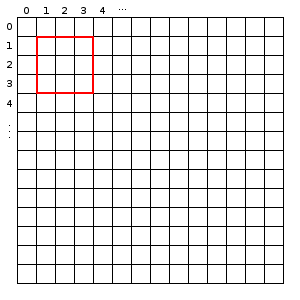
\includegraphics[scale=0.42,angle=0]{afsnit/vores_implementation/billeder/sloering/red_pixel_box}
    \end{center}
    \caption[]{Fra det originale billede trækkes en samling af
    $N\times{M}$ pixels ud omkring den aktuelle pixel. Her er $N = M =
    3$.}
    \label{red_box_nxm}
\end{figure}

\begin{figure}[!h]
    \renewcommand{\arraystretch}{1.8}
    \centering
    \begin{tabular}{|c|c|c|}
        \hline
     35 & 98  & 23 \\\hline
     48 & \cellcolor[gray]{0.5}42 & 0 \\\hline
     8  & 12   & 29 \\\hline
    \end{tabular}
    \caption[]{Værdier i et $N\times{}M$ vindue.}
    \label{median_kernel}
\end{figure}

\begin{figure}[!h]
    \renewcommand{\arraystretch}{1.5}
    \centering
    \begin{tabular}{|c|c|c|c|c|c|c|c|c|}
        \hline
     0 & 8 & 12 & 23 & \cellcolor[gray]{0.5}29 & 35 & 42 & 48 & 98\\\hline
    \end{tabular}
    \caption[]{Værdierne er sorteret og medianen er 29. Denne værdi
    erstatter den oprindelige værdi.}
    \label{median_array}
\end{figure}

\subsubsection*{Eksempler}
\begin{figure}[!h]
    \centering
    \subfloat[Original]{\label{simple_original}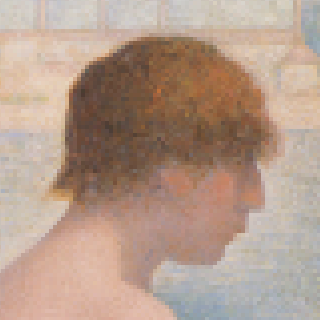
\includegraphics[angle=0,width=0.3\textwidth]{afsnit/vores_implementation/billeder/sloering/original}}\hspace{1em}
    \subfloat[$3 \times 3$ vindue]{\label{simple_3_3}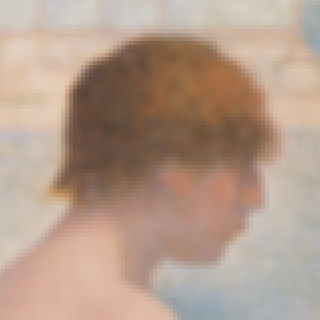
\includegraphics[angle=0,width=0.3\textwidth]{afsnit/vores_implementation/billeder/sloering/simple_3_3}}\hspace{1em}
    \subfloat[$7 \times 7$ vindue]{\label{simple_7_7}
\includegraphics[angle=0,width=0.3\textwidth]{afsnit/vores_implementation/billeder/sloering/simple_7_7}}
    \caption[]{\ref{simple_original}: Zoom af detajler i det originale
    billede. \ref{simple_3_3}: Median med et vindue på $3\times{}3$.
    Farverne er blevet mere ensartede mens kanterne stadig er skarpe.
    \ref{simple_7_7}: Median med et vindue på $7\times{}7$. Farverne er
    meget ensartede, men det ses at kanterne er blevet mere udvisket med
    det større vindue.}
    \label{simple_metode}
\end{figure}

\begin{figure}[!h]
    \centering
    \subfloat[Original]{\label{gaussian_original}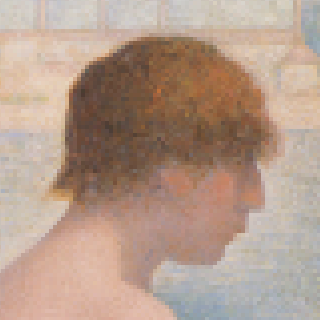
\includegraphics[angle=0,width=0.3\textwidth]{afsnit/vores_implementation/billeder/sloering/original}}\hspace{1em}
    \subfloat[$3 \times 3$ vindue]{\label{gaussian_3_3}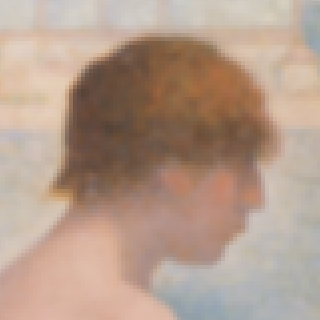
\includegraphics[angle=0,width=0.3\textwidth]{afsnit/vores_implementation/billeder/sloering/gaussian_3_3}}\hspace{1em}
    \subfloat[$7 \times 7$ vindue]{\label{gaussian_7_7}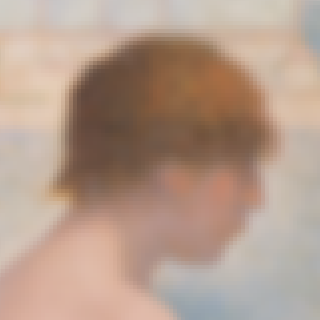
\includegraphics[angle=0,width=0.3\textwidth]{afsnit/vores_implementation/billeder/sloering/gaussian_7_7}}
    \caption[]{\ref{gaussian_original}: Zoom af detajler i det originale
    billede. \ref{gaussian_3_3}: Median med et vindue på $3\times{}3$.
    Farverne er blevet mere ensartede mens kanterne stadig er skarpe.
    \ref{gaussian_7_7}: Median med et vindue på $7\times{}7$. Farverne er
    meget ensartede, men det ses at kanterne er blevet mere udvisket med
    det større vindue.}
    \label{gaussian_metode}
\end{figure}

\begin{figure}[!h]
    \centering
    \subfloat[Original]{\label{median_original}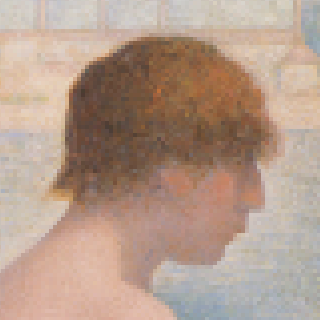
\includegraphics[angle=0,width=0.3\textwidth]{afsnit/vores_implementation/billeder/sloering/original}}\hspace{1em}
    \subfloat[$3 \times 3$ vindue]{\label{median_3_3}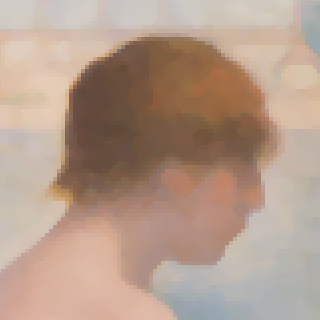
\includegraphics[angle=0,width=0.3\textwidth]{afsnit/vores_implementation/billeder/sloering/median_3_3}}\hspace{1em}
    \subfloat[$7 \times 7$ vindue]{\label{median_7_7}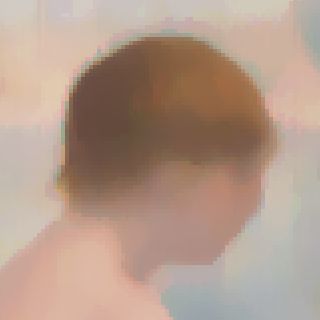
\includegraphics[angle=0,width=0.3\textwidth]{afsnit/vores_implementation/billeder/sloering/median_7_7}}
    \caption[]{\ref{median_original}: Zoom af detajler i det originale
    billede. \ref{median_3_3}: Median med et vindue på $3\times{}3$.
    Farverne er blevet mere ensartede mens kanterne stadig er skarpe.
    \ref{median_7_7}: Median med et vindue på $7\times{}7$. Farverne er
    meget ensartede, men det ses at kanterne er blevet mere udvisket med
    det større vindue.}
    \label{median_metode}
\end{figure}

}

% vim: set tw=72 spell spelllang=da:
